\newpage

\begin{multicols}{2}
\section{TIE HIGH}
\makebox[\linewidth]{\rule{0.5\textwidth}{0.4pt}}
{\bf Designer: } Martin Wearn\\
{\bf Cell Description: } A tie to Vdd cell.\\
\subsection*{Dimensions}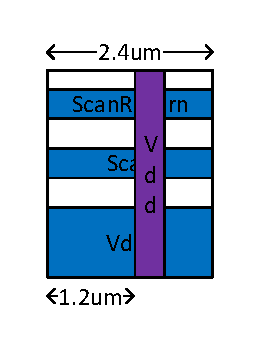
\includegraphics[width=\textwidth,height=4cm,keepaspectratio=true]{../tiehigh/blackbox.pdf}

\section{TIE LOW}
\makebox[\linewidth]{\rule{0.5\textwidth}{0.4pt}} 
{\bf Designer: } Martin Wearn\\
{\bf Cell Description: } A  tie to GND cell.\\
\subsection*{Dimensions}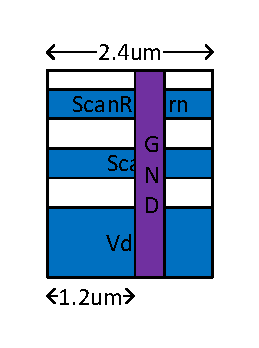
\includegraphics[width=\textwidth,height=4cm,keepaspectratio=true]{../tielow/blackbox.pdf}
\end{multicols}

\section{ROWCROSSER} \makebox[\linewidth]{\rule{\textwidth}{0.4pt}}
{\bf Designer: } Martin Wearn\\
{\bf Cell Description: } A row crossing cell.\\
\subsection*{Dimensions}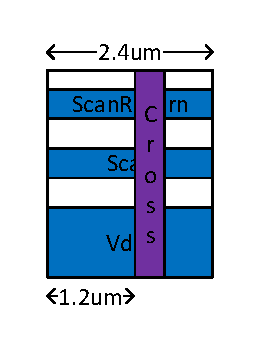
\includegraphics[width=\textwidth,height=4cm,keepaspectratio=true]{../rowcrosser/blackbox.pdf}



